\documentclass[twocolumn]{article}
\usepackage{xeCJK}
\setCJKmainfont{IPA明朝}
\usepackage[a4paper, top=1in, bottom=1in, left=2cm, right=2cm]{geometry}
\usepackage[singlespacing]{setspace}
\usepackage{amsmath}
\usepackage{amssymb}
\usepackage{graphicx}
\usepackage{hyperref}
\usepackage[font=small,labelfont=bf]{caption}
\title{水中の鉛筆が描くアストロイド:\\光と幾何学の不思議な出会い}
\author{M. Ryu \\ {\href{mailto:mingshey@hafs.hs.kr}{mingshey@hafs.hs.kr}}}
\renewcommand{\figurename}{図}
\begin{document}
\maketitle
\section{序論}

水に部分的に浸かった鉛筆が曲がって見える現象は、光の屈折を学ぶ初期段階でよく見かける現象です(図\ref{fig:pencil})。しかし、鉛筆の先端の見かけの位置が観察角度によって変化する現象は、より深い分析が必要です。

\begin{figure}[ht]
	\centering
	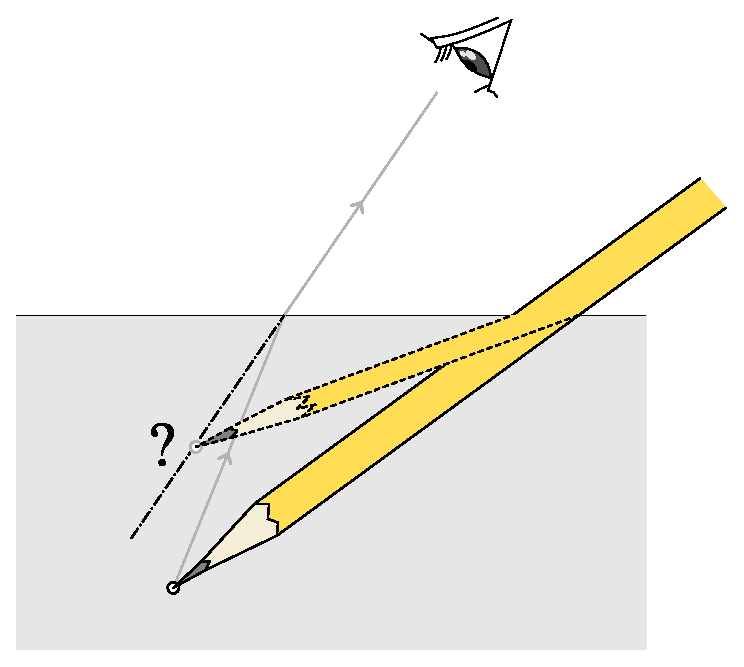
\includegraphics[width=2in]{figs/g164.eps}
	\caption{水中に折れ曲がってみえる鉛筆}
	\label{fig:pencil}
\end{figure}

一般的に物理学の入門課程では、真上から見たときの見かけの深さについて学ぶことが多いですが、斜めから見たときの見かけの位置の変化については、詳細な議論は省略されることが多いです。高度な光学の教科書でも、この現象は簡単に触れられるか、省略されることが多いです。

これは、この現象が比較的複雑な数学的な処理を要求するため、入門課程で扱うには適しておらず、一方で、レンズや鏡のような光学機器の動作原理に比べて、相対的に重要性が低いと評価されるため、高度な課程で扱うにも適さないためでしょう。

しかし、このように単純に見える現象でも、時には好奇心を刺激します。筆者以外にも多くの人がこの現象について疑問に思ったことでしょう。本稿では、このような疑問に対する答えを示したいと考えています。

\section{簡単な解答}

興味はあるが、あまり時間をかけたくない読者のために結論から述べると、平らな水面下の点光源を水面上から見ると、像の位置は視点によって変化する。視点が動くにつれて法平面内で観察される像の軌跡は、一種のコースティクス曲線であり、この場合、変形したアストロイドと呼ばれる曲線となる。

図\ref{fig:caustic}のように、物体と視点を含む法平面において、法平面と水面の交線を$x$軸、物体を通り法線となる直線を$y$軸とすると、像の軌跡は次の曲線の一部となる。
$$ \left| \dfrac{x}{M} \right| ^ {2/3} 
+ \left| \dfrac{y}{N} \right| ^ {2/3} = 1,$$
ここで、$M = D/\sqrt{n^2 - 1}$は全反射の臨界角($\theta_{\mathrm{c}}$)によって決まる入射距離の最大値であり、
$N = D/n$は真上から観察したときの物体の見かけの深さ、
$D$は物体の実際の深さ、$n$は空気に対する水の屈折率である。

\begin{figure}
	\centering
	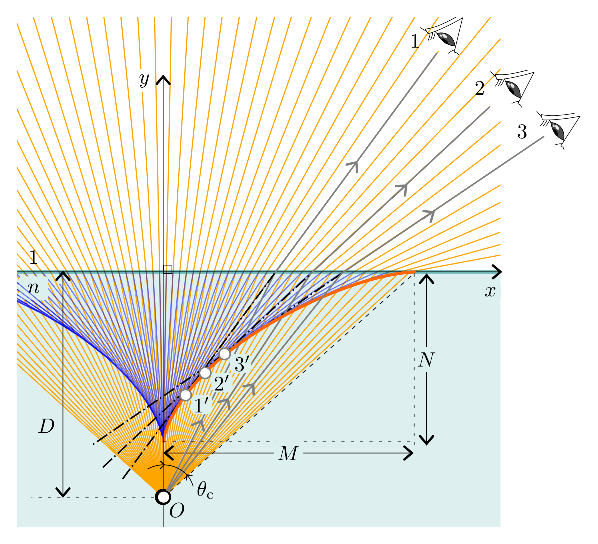
\includegraphics[width=3in]{figs/g409.eps}
	\caption{視点によって位置が変化する像の軌跡}
	\label{fig:caustic}
\end{figure}
	
\section{式の導出}

空気と水の屈折率をそれぞれ$n_1$および$n_2$とする。空気と水の境界面の下、深さ$D$の位置に点物体$\mathrm{O}$があるとする。物体から出た光線が$y$軸から$a$だけ離れた境界面上の点Aに、法線から$\theta_2$の角度で入射し、同じ法線から$\theta_1$の角度で空気中に屈折する。

屈折光線の延長線は$y$軸と点B$(0, b)$で交わる。入射角$\theta_2$が変化するとき、直線${\mathrm{AB}}$が重なり合い包絡線を形成し、このように光線が集まってできる包絡線をコースティクス曲線(caustic)と呼ぶ。\footnote{この場合、実際の光線ではなく、光線の延長線が作る仮想的なコースティクス、すなわち虚コースティクスである。} 像は線分${\mathrm{AB}}$とコースティクスの接点$\mathrm{C}$に位置する。これは、この点の近傍の光線束が局所的に発散する点だからである。

\begin{figure}
	\centering
	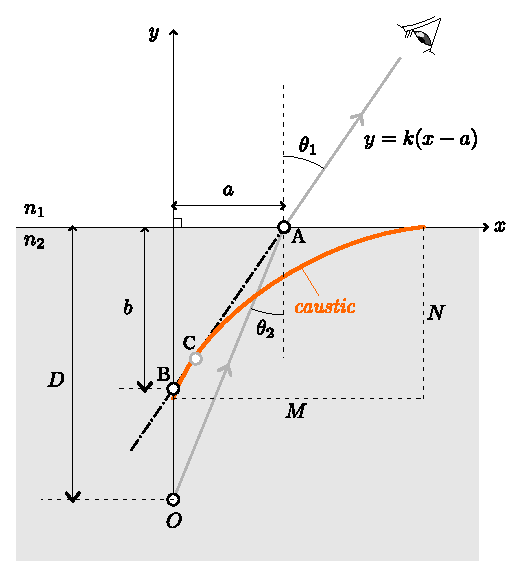
\includegraphics[width=3in]{figs/g237.eps}
	\caption{空気と水の界面での光の屈折と、その延長線とコースティクスの幾何学的関係}
	\label{fig:geometry}
\end{figure}
	
直線ABは$y$軸からの入射点までの距離$a$を媒介変数とする以下の式で表される。
$$y=k(x-a).$$
ここで、直線の傾き$k$はスネルの法則
$ {n_1} \sin\theta_1 = {n_2} \sin\theta_2$、または$\sin\theta_1 = n\sin\theta_2$
より、
$$k=\dfrac{1}{\tan\theta_1}=\dfrac{\cos\theta_1}{\sin\theta_1}
=\dfrac{\sqrt{1-n^2\sin^2\theta_2}}{n\sin\theta_2}.$$
幾何学的に以下の関係が成り立つ。
$$\begin{aligned}
	a &= D\tan\theta_2 = \dfrac{D\sin\theta_2}{\cos\theta_2},\\
	b &= -ka \\
	&= -\dfrac{D\sin\theta_2}{\cos\theta_2}
	\dfrac{\sqrt{1-n^2\sin^2\theta_2}}{n\sin\theta_2}\\
	&=-\dfrac{D\sqrt{1-n^2\sin^2\theta_2}}{n\cos\theta_2}.
\end{aligned}$$
ここで、無次元パラメータ$\alpha=a/M$および$\beta=b/N$を導入すると、
$$ \begin{aligned}
	\alpha^2 + \beta^2 &= \dfrac{a^2}{M^2}+\dfrac{b^2}{N^2}\\
	&=\dfrac{n^2-1}{D^2}\dfrac{D^2\sin^2\theta_2}{\cos^2\theta_2}%
	+\dfrac{n^2}{D^2}\dfrac{D^2(1-n^2\sin^2\theta_2)}{n^2\cos^2\theta_2}\\
	&=\dfrac{\left(n^2-1\right)\sin^2\theta_2 + 1-n^2\sin^2\theta_2}
	{\cos^2\theta_2}\\
	&=\dfrac{1-\sin^2\theta_2}{\cos^2\theta_2}\\
	&= 1
\end{aligned}$$
	
また、無次元座標 $\xi=x/M$ および $\eta=y/N$ を導入すると、視点が $xy$ 平面上で移動するにつれて、点 $\mathrm{A}(a, 0)$ と $\mathrm{B}(0, b)$ も移動する。このとき、点 $\mathrm{A}$, $\mathrm{B}$ にそれぞれ対応する $\xi\eta$ 平面上の点 $\mathrm{A'}(\alpha, 0)$ と $\mathrm{B'}(0, \beta)$ は、距離が 1 で一定となるように移動する。

パラメータ $\alpha$ を持つ直線 ${\mathrm{A'B'}}$ の包絡線は、よく知られたアストロイド(\emph{astroid}、小惑星を意味する \emph{asteroid} と混同しないこと)と呼ばれる曲線で、以下の式で表される(付録 \ref{app:astroid} 参照)。
$$ \left| \xi \right|^{2/3} + \left| \eta \right|^{2/3} = 1. $$

\begin{figure}
	\centering
	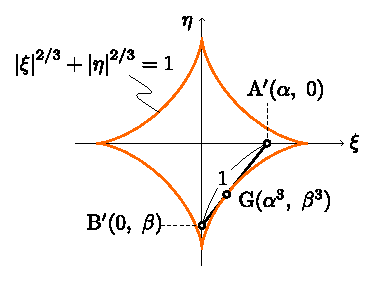
\includegraphics{figs/g107.eps}
	\caption{$\xi\eta$ 平面への投影で得られるコースティクスは、アストロイドである。}
	\label{fig:astroid}
\end{figure}

直線 ${\mathrm{A'B'}}$ とアストロイドの接点は $\mathrm{G}(\alpha^3, \beta^3)$ であり、この点が像の位置 $\mathrm{C}$ に対応する。
	
したがって、以下の関係式から像の座標 $(x_{\mathrm{C}}^{}, y_{\mathrm{C}}^{})$ を得ることができる。
$$ \left\{ 
\begin{aligned}
	\xi_{\mathrm{G}}^{} &= \dfrac{x_{\mathrm{C}}^{}}{M} = \alpha^3 = \dfrac{a^3}{M^3},\\
	\eta_{\mathrm{G}}^{} &= \dfrac{y_{\mathrm{C}}^{}}{N} = \beta^3 = \dfrac{b^3}{N^3}.
\end{aligned}
\right.$$
つまり、
$$ \left\{ 
\begin{aligned}
	x_{\mathrm{C}}^{} &= \dfrac{a^3}{M^2},\\
	y_{\mathrm{C}}^{} &= \dfrac{b^3}{N^2}=-\dfrac{k^3a^3}{N^2}.
\end{aligned}
\right.$$

ここで、
$\sin\theta_2 = {a}/{\sqrt{D^2+a^2}}$
を用いて
$$k = \dfrac{\sqrt{D^2-(n^2-1)a^2}}{na},$$
を得ることができ、
像の位置を$a$をパラメータとする関数として導出できる。
$$ \left\{ 
\begin{aligned}
	x_{\mathrm{C}}^{} &= (n^2-1)\dfrac{a^3}{D^2},\\
	y_{\mathrm{C}}^{}
	% 	&= -\dfrac{n^2}{D^2}\dfrac{a^3}
	%	{n^3a^3}\left\{ D^2-(n^2-1)a^2 \right\}^{3/2}\\
	&= -\dfrac{D}{n}\left\{ 1-(n^2-1)\dfrac{a^2}{D^2} \right\}^{3/2}.
\end{aligned}
\right.$$
	
\section{観測者が水中にある場合}

\begin{figure}
	\centering
	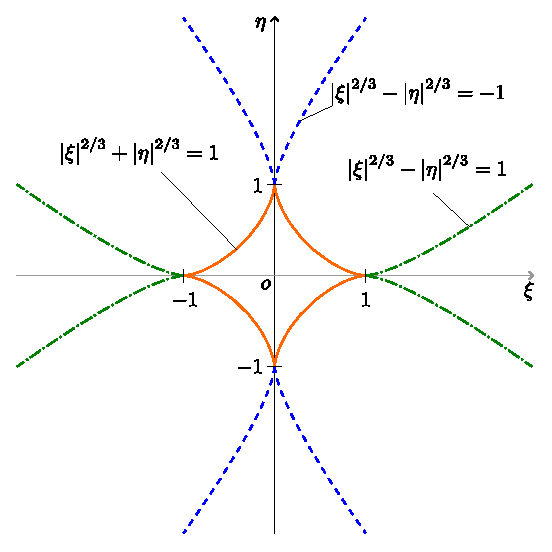
\includegraphics[width=3in]{figs/g254.eps}
	\caption{アストロイドと双曲-アストロイド}
	\label{fig:hyperastroid}
\end{figure}

物体が境界面から高さ$D$の空気中にあり、観測者が水中にある場合、相対的な屈折率は$1/n < 1$となり、同様の推論により、コースティクスに関する以下の式を得る(付録\ref{app:hyperastroid}参照)。
$$ \left| \xi \right|^{2/3} - \left| \eta \right|^{2/3} = -1, $$
ここで、$\xi = {x}/{W} $、$\eta = {y}/{Z}$ とおき、$W = {nD}/{\sqrt{n^2-1}}$、$Z = nD$ とすると、この曲線は漸近線を持たないが、$x \to \pm \infty$ のとき、傾きは $\pm Z/W = \pm \sqrt{n^2-1}$ に収束する。

したがって、水中から見た水面上の空は、鉛直線から全反射の臨界角内側の円(または円錐)内に圧縮されて見える。これは、スネルの窓(Snell's window)と呼ばれるよく知られた現象であり、全天写真など超広角写真に用いられる\href{https://ja.wikipedia.org/wiki/%E9%AD%9A%E7%9C%BC%E3%83%AC%E3%83%B3%E3%82%BA}{魚眼レンズ}(fisheye lens)の視野とも似ている。

この曲線は、より一般的には
$$ \left| \xi \right|^{r} - \left| \eta \right|^{r} = \pm1 $$
で表される曲線族に属し、\href{http://dynamicmathematicslearning.com/super-ellipse.html}{DML}\footnote{\ttfamily{dynamicmathematicslearning.com/super-ellipse.html}}ではスーパー双曲線(\emph{Super Hyperbola})と呼ばれ、\href{https://old.nationalcurvebank.org/superconicncb/superconicncb.htm}{National Curve Bank}\footnote{\ttfamily{https://old.nationalcurvebank.org/superconicncb/\\superconicnb.htm}}ではアストロイドが属する
$$ \left| \xi \right|^{r} + \left| \eta \right|^{r} = 1. $$
のような曲線族であるスーパー楕円(\emph{superellipse})とまとめてスーパー円錐曲線(\emph{superconics})と呼ばれる、広範な曲線族の一部である。

特に $r = 2/3$ の場合、
$$ \left| \xi \right|^{2/3} - \left| \eta \right|^{2/3} = \pm1 $$
という特殊な場合、空気中から水中に入射する光線のコースティクス曲線として物理学的に意味を持つ。この曲線はアストロイドとの関係が双曲線と楕円の関係に似ていることから、「双曲アストロイド」(\emph{hyperastroid})と呼ぶこともできるだろう。
	
\section{像の位置を求める}

物体の位置と視点が与えられたとき、コースティクスを利用して像の位置を以下のように求めることができる。

\begin{figure}[!h]
	\centering
	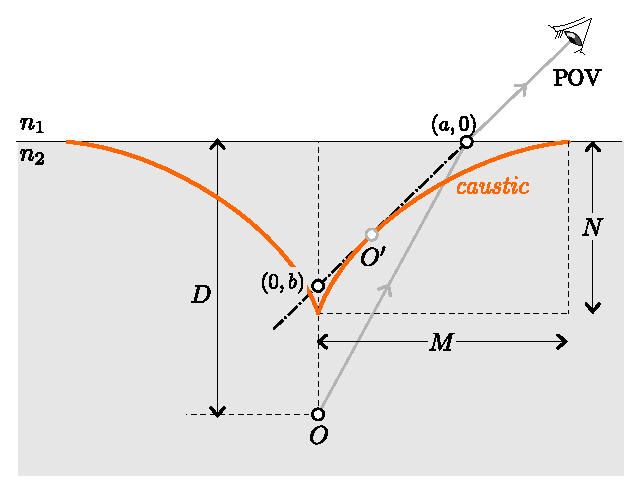
\includegraphics[width=2.7in]{figs/g394.eps}
	\caption{コースティクスを利用した像の位置決定}
	\label{fig:image_caustic}
\end{figure}

図\ref{fig:image_caustic}のように、視点(POV)からコースティクスに接線を引く。接線とコースティクスの接点($\mathrm{O'}$)が像の位置であり、接線が水面と交わる点が物体($\mathrm{O}$)から出た光線が空気との界面に入射する点である。

視点(POV)の座標を$(x_{\mathrm{V}}^{}, y_{\mathrm{V}}^{})$、物体($\mathrm{O}$)の座標を$(x_{\mathrm{O}}^{}, y_{\mathrm{O}}^{})$、求める像($\mathrm{O'}$)の座標を$(x_{\mathrm{O'}}^{}, y_{\mathrm{O'}}^{})$とする。屈折光線が水面および$\mathrm{O}$を通る法線(ここでは$y$軸)と交わる点をA, Bとし、それぞれの座標を$(a, 0)$, $(0, b)$とする。

このとき、$\xi\eta$座標系における対応する点は、それぞれ、視点: $(\xi_{\mathrm{V}}^{}, \eta_{\mathrm{V}}^{})=(x_{\mathrm{V}}^{}/M, y_{\mathrm{V}}^{}/N)$、物体: $(\xi_{\mathrm{O}}^{}, \eta_{\mathrm{O}}^{})=(x_{\mathrm{O}}^{}/M, y_{\mathrm{O}}^{}/N)$、像: $(x_{\mathrm{O'}}^{}/M, y_{\mathrm{O'}}^{}/N)=(\alpha^3, \beta^3)$であり、$\mathrm{A'}$, $\mathrm{B'}$の座標はそれぞれ$(\alpha, 0) = (a/M, 0)$, $(0, \beta) = (0, b/N)$である。ここで、$M=D/\sqrt{n^2-1}$, $N=D/n$, $D=y_{\mathrm{O}}^{}$である。

接線と水面、$\eta$軸が作る比例関係から、以下の式を得る。
$$\dfrac{\eta_{\mathrm{V}}^{}}{\xi_{\mathrm{V}}^{}-\alpha}=-\dfrac{\beta}{\alpha}.$$

ここで、$\beta = \pm \sqrt{1-\alpha^2}$ を用い、両辺を二乗して整理すると、$\alpha$ に関する4次方程式
\[
\left( 1 - \alpha^2 \right) \left(\alpha-\xi_{\mathrm{V}} \right)^2 = \alpha^2 \eta_{\mathrm{V}}^2
\]
を得る。一般に、4次方程式は4つの複素数解を持つが、この場合、実数解が2つ存在する。求めたい$\alpha$の値は、0と$\xi_{\mathrm{V}}$の間にあるものとなる。4次方程式を手計算で解くことは一般的に困難である。コンピュータ代数システム (CAS) を利用して解析解を求めることも可能であるが、数値解法を用いて近似解を求める方が効率的なことが多い。 (付録 \ref{app:python} 参照)

方程式の形式からわかるように、像の座標は視点の座標に依存する。例えば、水中に半分浸かった鉛筆の先端は、図\ref{fig:pencil_view}のように、視点$1$, $2$によってそれぞれ$1'$, $2'$の位置に異なる。
	
\begin{figure}[h]
	\centering
	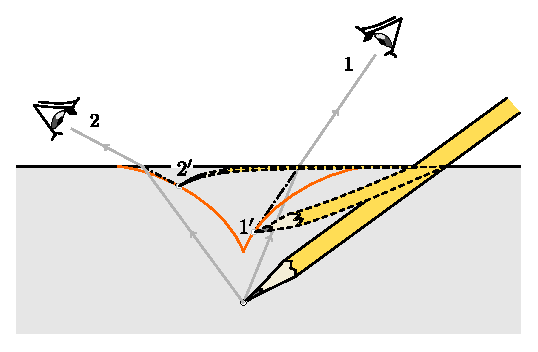
\includegraphics[width=2.4in]{figs/g43.eps}
	\caption{水中に浸かった鉛筆の像。視点が$1$, $2$と変化すると、鉛筆の先端の像の位置もそれぞれ$1'$, $2'$と変化する。}
	\label{fig:pencil_view}
\end{figure}

水中に連続した物体がある場合、図\ref{fig:extended_image}のように、物体の表面に沿って配置された点$1, 2, 3, ...$に対して、それぞれ同じ方法で像$1', 2', 3', ...$を求めることができる。点が連続的に移動するとき、それに伴って移動する像の軌跡が、物体の像となる。

\begin{figure}[h]
	\centering
	\includegraphics*[width=2.5in]{figs/g242.eps}
	\caption{連続的な物体の像。物体上の点$1, 2, 3, ...$に対応する像の位置$1', 2', 3', ...$を連続的に結ぶことで、全体の像を描くことができる。}
	\label{fig:extended_image}
\end{figure}

\begin{figure}[h]
	\centering
	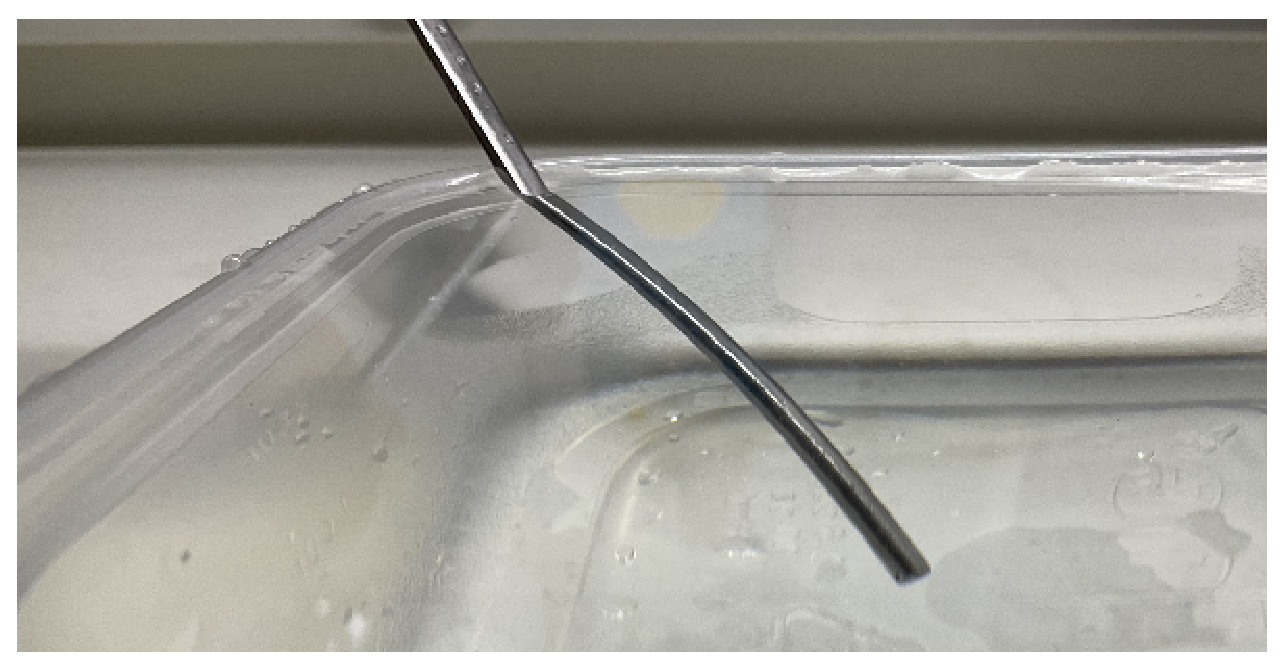
\includegraphics[width=3in]{figs/img_1805_2.eps}
	\caption{水に半分浸かった箸の写真。水面に近い低い角度から撮影}
	\label{fig:picture}
\end{figure}
	
別の方法として、フェルマーの原理を用いて光線が水面に入射する点を求め、この点をアストロイドの接点の式に代入することで像の位置を決定できる。
入射点の$x$座標は、
\[
\dfrac{n_1 \left( x - x_{\mathrm{V}}^{} \right)}{\sqrt{ y_{\mathrm{V}}^2 + \left( x - x_{\mathrm{V}}^{} \right)^2 }}
+\dfrac{n_2 \left( x - x_{\mathrm{O}}^{} \right)}{\sqrt{ y_{\mathrm{O}}^2 + \left( x - x_{\mathrm{O}}^{} \right)^2 }}
= 0,
\]
または、これを整理した4次方程式
\[ \begin{aligned}
	\left( x - x_{\mathrm{V}}^{} \right)^2 & \left\{ y_{\mathrm{V}}^2 + \left(x - x_{\mathrm{V}}^{} \right)^2 \right\}\\
	&= n^2 \left( x - x_{\mathrm{O}}^{} \right)^2 \left\{ y_{\mathrm{V}}^2 + \left(x - x_{\mathrm{V}}^{} \right)^2 \right\}
\end{aligned}
\]
の解のうち、$x_{\mathrm{O}}^{}$と$x_{\mathrm{V}}^{}$の間の実数解として与えられる。この場合も、厳密な解析解を求めるよりも、数値解法を用いて近似解を求める方が実用的である。

像の位置を求めるPythonの例は、
\href{https://github.com/mingshey/python_projects/blob/main/Refraction_Image_en.ipynb}%
{\sffamily{github}}\footnote{\ttfamily{https://github.com/mingshey/python\_projects/blob/main/\\Refraction\_Image\_en.ipynb}} に公開されている。

\section{水中空間の像}

前節で像の位置を定量的に求める方法を学んだので、この方法を用いて、水中空間を空気中から見たときの像がどのように歪んで見えるかを調べてみよう。図\ref{fig:grid_underwater}のように正方形格子で表された水中の長方形領域は、空気中から見下ろすとき、視点の相対的な高さによって図\ref{fig:image_underwater}〜\ref{fig:seashell}のように見える。

\begin{figure}[!h]
	\centering
	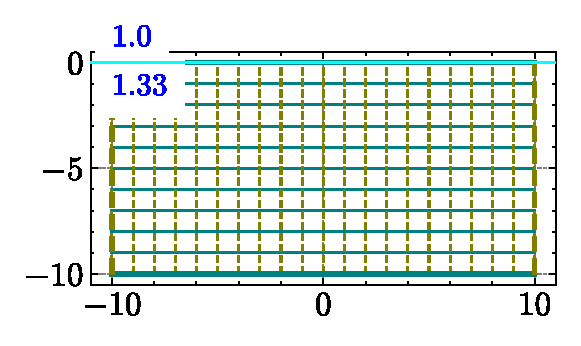
\includegraphics[width=2.7in]{figs/grid_underwater.eps}
	\caption{水中の格子状物体}
	\label{fig:grid_underwater}
\end{figure}

\begin{figure}[!t]
	\centering
	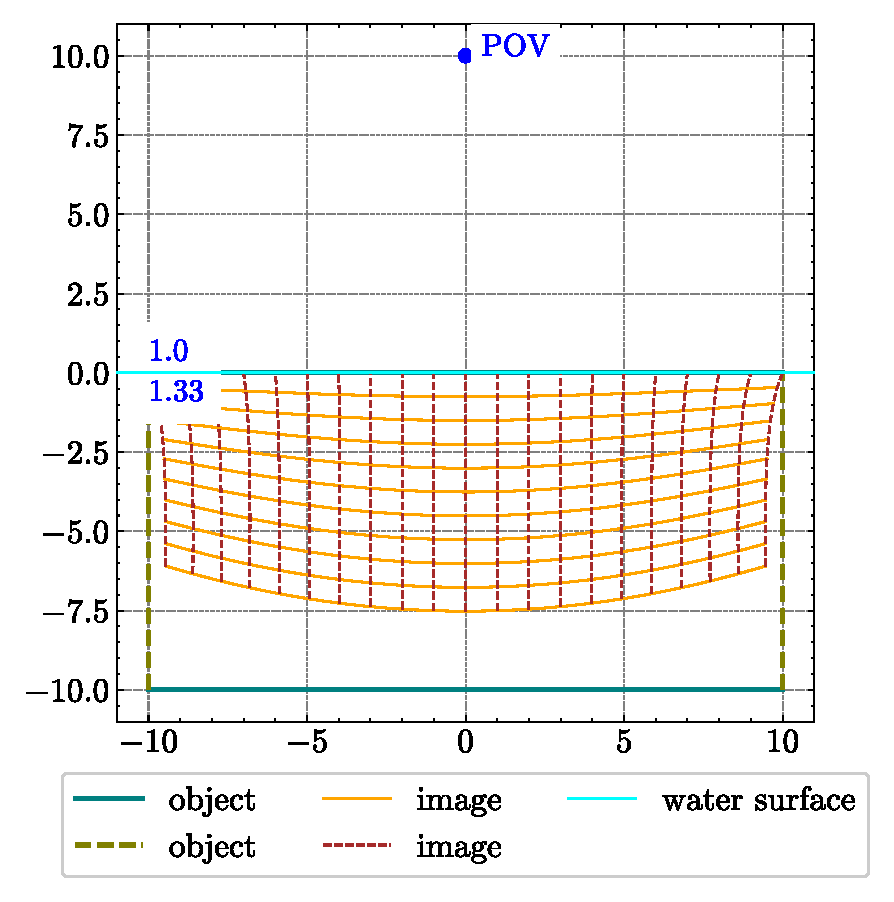
\includegraphics[width=3in]{figs/image_underwater1.eps}
	\caption{格子の像。観察者の目の高さが水面とほぼ同じかそれよりも高い場合、像は屈折率にほぼ等しい比率で全体的に平坦に見えます。\ref{fig:image_underwater}$\sim$\ref{fig:snell_window}では比較のためにグリッドの外形を長方形で示しています。}
	\label{fig:image_underwater}
\end{figure}

\begin{figure}[!t]
	\centering
	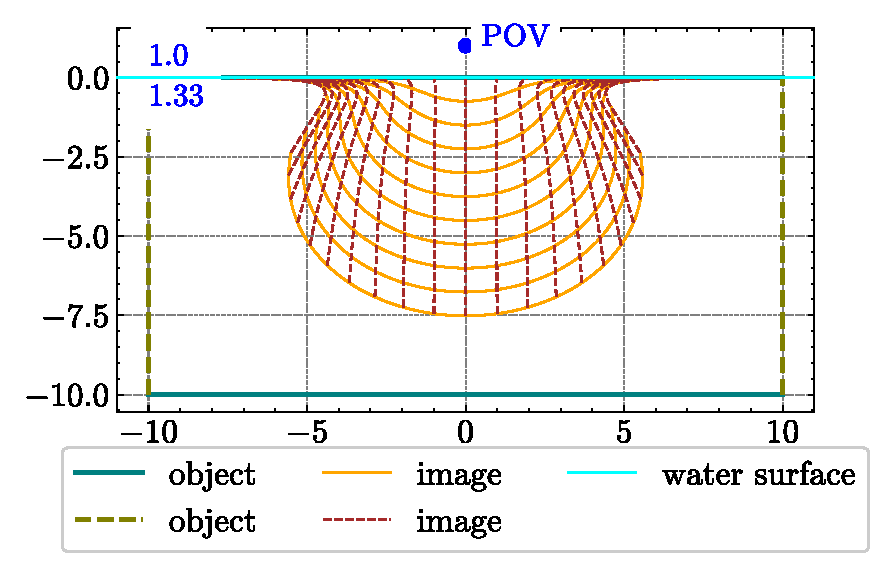
\includegraphics[width=3in]{figs/fishjar.eps}
	\caption{格子の像。視点の高さが水の深さより非常に低いとき、長方形の空間が魚鉢のような形に圧縮されて見える。}
	\label{fig:fishbowl}
\end{figure}

\begin{figure}[!t]
	\centering
	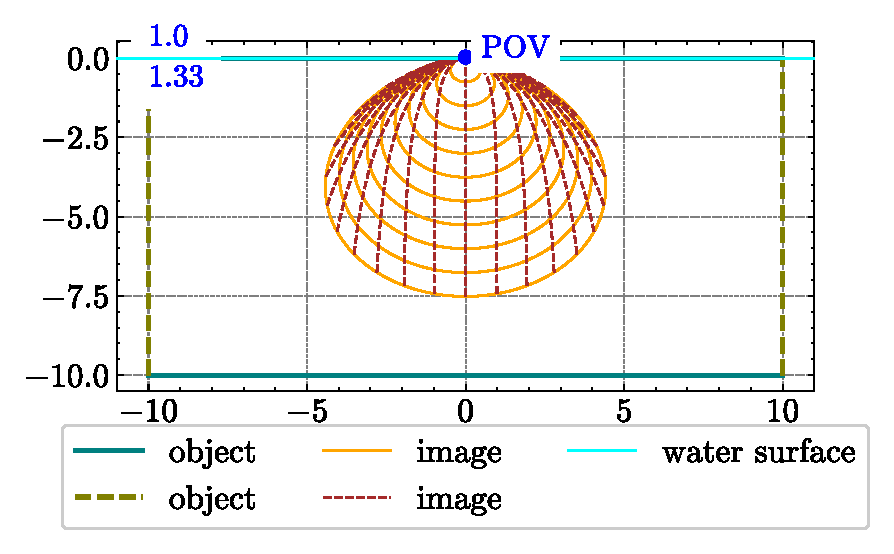
\includegraphics[width=3in]{figs/seashell_shape.eps}
	\caption{格子の像。視点が水面に極めて近いとき、長方形の空間が貝殻のような形に圧縮されて見える。}
	\label{fig:seashell}
\end{figure}

水面に接する空気中に同じ形状の格子を置いたとき、水中から見た格子の見かけは図\ref{fig:snell_window}のように、全反射の臨界角を境界とする円錐の内側に圧縮されて見える。水面がこの円錐を切る円をスネルの窓と呼び、水面上の空の風景はすべてスネルの窓の中に圧縮されて見える。スネルの窓の真上空は歪みが少なく、屈折率の比に応じて遠ざかって見える傾向がある一方、それ以外の空間は視野角が圧縮され、距離が遠ざかるように歪む。特に、水面に近いほど歪みが大きいことが分かる。

\begin{figure}
	\centering
	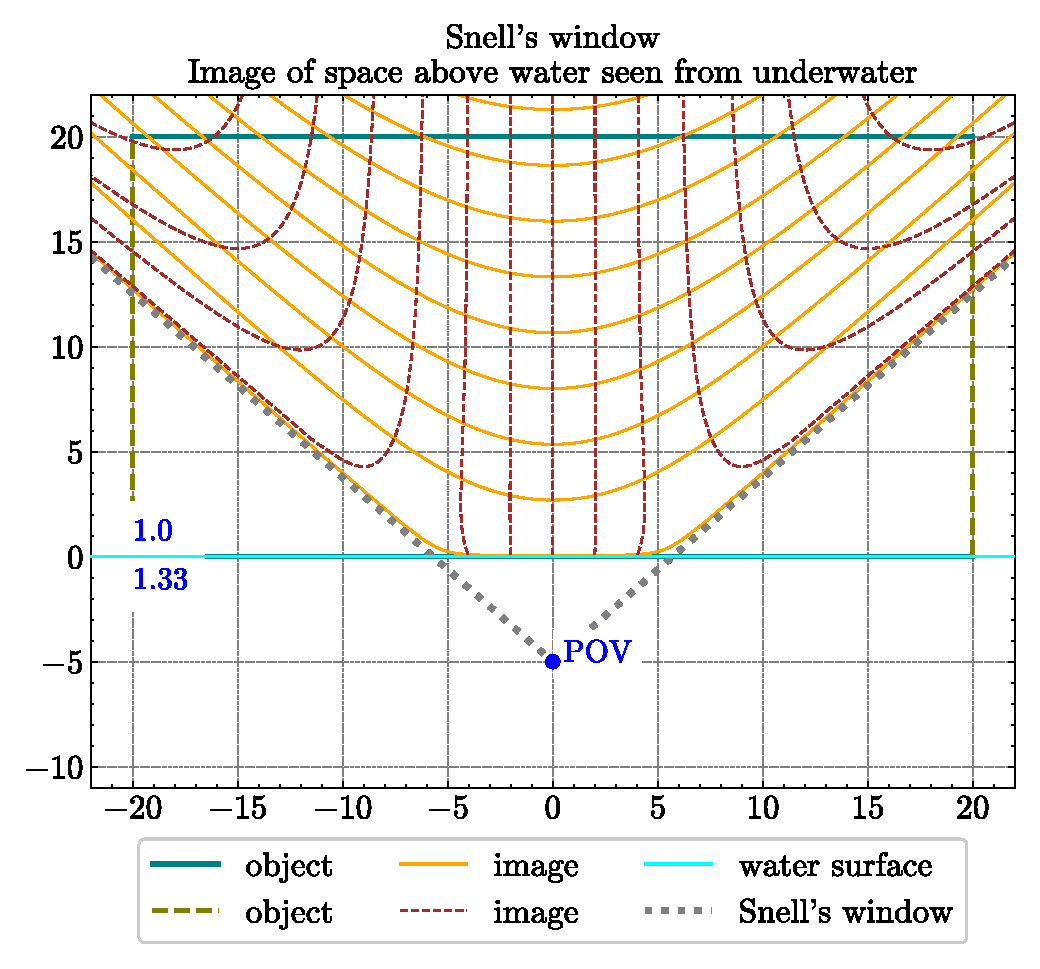
\includegraphics[width=3.3in]{figs/snell_window.eps}
	\caption{スネルの窓。水中から水面上の空間を見るときの像の様子。スネルの窓を定義する円錐の母線を便宜上Snell's windowと表記する。}
	\label{fig:snell_window}
\end{figure}

	
\appendix
\newcommand{\pd}[2]{{\frac{\partial #1}{\partial #2}}}
\newcommand{\ilpd}[2]{{{\partial #1}/{\partial #2}}}
\section{包絡線としてのアストロイド} \label{app:astroid}
$xy$平面上で、$x$軸上の点$(a, 0)$と$y$軸上の点$(0, b)$が一定の距離$c$を保ちながら動くとする。このとき、両点を結ぶ直線の式は
$$y=-\dfrac{b}{a}(x-a)$$
となる。ここで、$b=\pm \sqrt{c^2-a^2}$を代入すると、
$$y(x, a) = \mp \dfrac{\sqrt{c^2-a^2}}{a}(x-a)$$
となる。
$a$の値を変化させると、二点を結ぶ直線も変化する。これらの直線の包絡線は、$a$が微小に変化しても変わらない定点、すなわち$\ilpd{y}{a} = 0$となる点の軌跡として定義できる。この条件を満たす$(x, y)$を求めるために、$y$を$a$で微分すると、

$$ \begin{aligned}
	\pd{y}{a} &= \pm\left[\left( \dfrac{1}{\sqrt{c^2-a^2}}+\dfrac{\sqrt{c^2-a^2}}{a^2}\right) (x-a) + \dfrac{\sqrt{c^2-a^2}}{a} \right]\\
	&= \pm \dfrac{(a^2+c^2-a^2)(x-a)+a(c^2-a^2)}{a^2\sqrt{c^2-a^2}}\\
	&= \pm \dfrac{c^2 x - a^3}{a^2 \sqrt{c^2 - a^2}}\\
	&= 0.
\end{aligned}
$$
よって、定点の$x$座標は$x = a^3/c^2$であり、これを$y(x, a)$に代入すると$y$座標の値は
$$ \begin{aligned}
	y(x, a) &= \mp \dfrac{\sqrt{c^2-a^2}}{a}\left(\dfrac{a^3}{c^2}-a\right)\\
	& = \pm \dfrac{\left( c^2- a^2 \right)^{3/2}}{c^2}\\
	& = \dfrac{b^3}{c^2}
\end{aligned}
$$
となる。したがって、定点の座標$(x, y)$は、以下のアストロイドの式を満たす。
$$ \left|\dfrac{x}{c}\right|^{2/3} + \left|\dfrac{y}{c}\right|^{2/3} = 1. $$

\section{双曲アストロイド}\label{app:hyperastroid}
本稿で命名した「双曲アストロイド」は、$x$軸上の点A$(a, 0)$と$y$軸上の点B$(0, b)$が以下の関係を満たしながら動くとき、両点を結ぶ直線の包絡線として定義できる。
$$b^2-a^2=c^2$$
このとき、包絡線の方程式は次の双曲アストロイドの方程式となる。
$$ \left|\dfrac{x}{c}\right|^{2/3} - \left|\dfrac{y}{c}\right|^{2/3} = -1. $$
導出過程は付録\ref{app:astroid}と同様であるため、ここでは省略する。
ここで、点Aから包絡線に接線を引くと、接点の座標は$(-a^3/c^2, b^3/c^2)$で与えられる。

任意の視点$(x_{\mathrm{V}}, y_{\mathrm{V}})$から双曲アストロイドに接線を引いたとき、接線が$x$軸と交わる点を$(a,0)$とすると、$a$は次の4次方程式
$$ \left( a^2 + c^2 \right) \left(a - x_{\mathrm{V}} \right)^2 = a^2 y_{\mathrm{V}}^2$$
の実根のうち、$0$と$x_{\mathrm{V}}$の間にある値であり、このとき$b = \pm \sqrt{a^2 + c^2}$となる。

\section{アストロイドの接線を利用した像の位置を求めるPythonコード} \label{app:python}
\begin{verbatim}
	import numpy as np
	import sympy as sym
	from scipy.optimize import root
	
	ksi, eta, alfa = sym.symbols('xi eta alpha')
	eqn = (alfa - ksi)**2 * (1 - alfa**2)\
	    - alfa**2 * eta**2
	eqnf = sym.lambdify((ksi, eta, alfa), eqn);
	
	def imgloc(pov, obj, nrel):
	xv, yv = pov
	xo, yo = obj
	M = yo / np.sqrt(nrel**2 - 1)
	N = yo / nrel
	xi_v = (xv - xo) / M
	eta_v = yv / N
	alpha = root(lambda x: eqnf(xi_v, eta_v, x),\
	    xi_v).x[0]
	beta = np.sqrt(1 - alpha**2)
	xim = alpha**3 * M + xo
	yim = beta**3 * N
	xpoi = (xim*yv - yim*xv)/(yv - yim)
	
	img = np.array([xim, yim])
	poi = np.array([xpoi, 0])
	
	return img, poi
\end{verbatim}

\section*{}
\vfill
	

\noindent
本稿は韓国語で執筆され、翻訳にはGoogleのGemini言語モデルが活用されました。
%	
%	\section*{}
%	
%	\noindent
%	娘には、いつも的確で心のこもったアドバイスをもらい、大変助かりました。心から感謝申し上げます。
	
%\end{japanese}
\end{document}